\section{Covariance Matrices}
Covariance Matrices (Variance-Covariance Matrices), are used to depict the uncertainty of variables and the correlation between the uncertainty of variables, and are an integral component to least squares.  The visualization and calculation of the covariance matrices will be covered later, but this section is to introduce the general concept of a covariance matrix.  For example:

Lets say you are standing at point (0,0) in a local coordinate system.  Using a compass you determine that a tree is located at about a 45 degree azimuth from true north, and about 100 meters away.  Using trigonometry, you can report the coordinate using the equations:
\begin{align*}
x_{tree} &= d \cos(az) \\
y_{tree} &= d \sin(az)
\end{align*}

\begin{figure}[H]
	\centering
	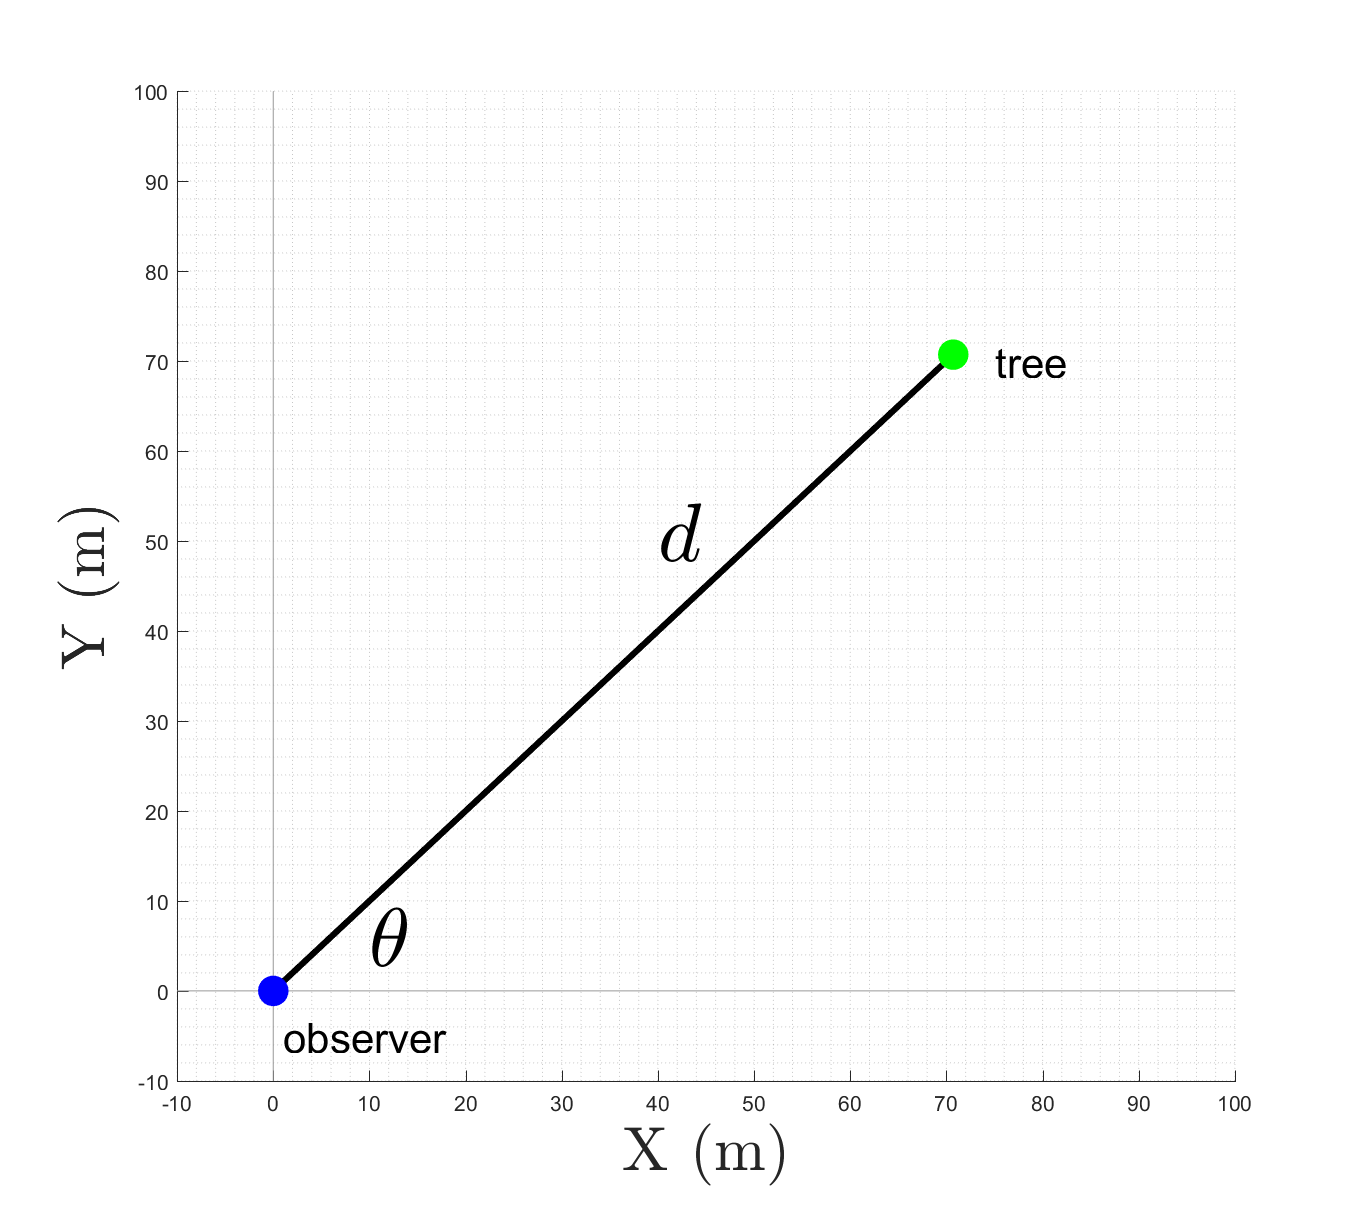
\includegraphics[height = 3in]{treefig.png}
\end{figure}

If you determined that you had some uncertainty in your measurements:

\begin{align*}
d \pm \sigma_d &= 100m \pm 10m \\
az \pm \sigma_{az} &= 45\degree  \pm 1\degree
\end{align*}

The estimate for the position of the tree would look something like the following figure, because there is much more uncertainty in the distance measurement than the angle measurement.

\begin{figure}[H]
	\centering
	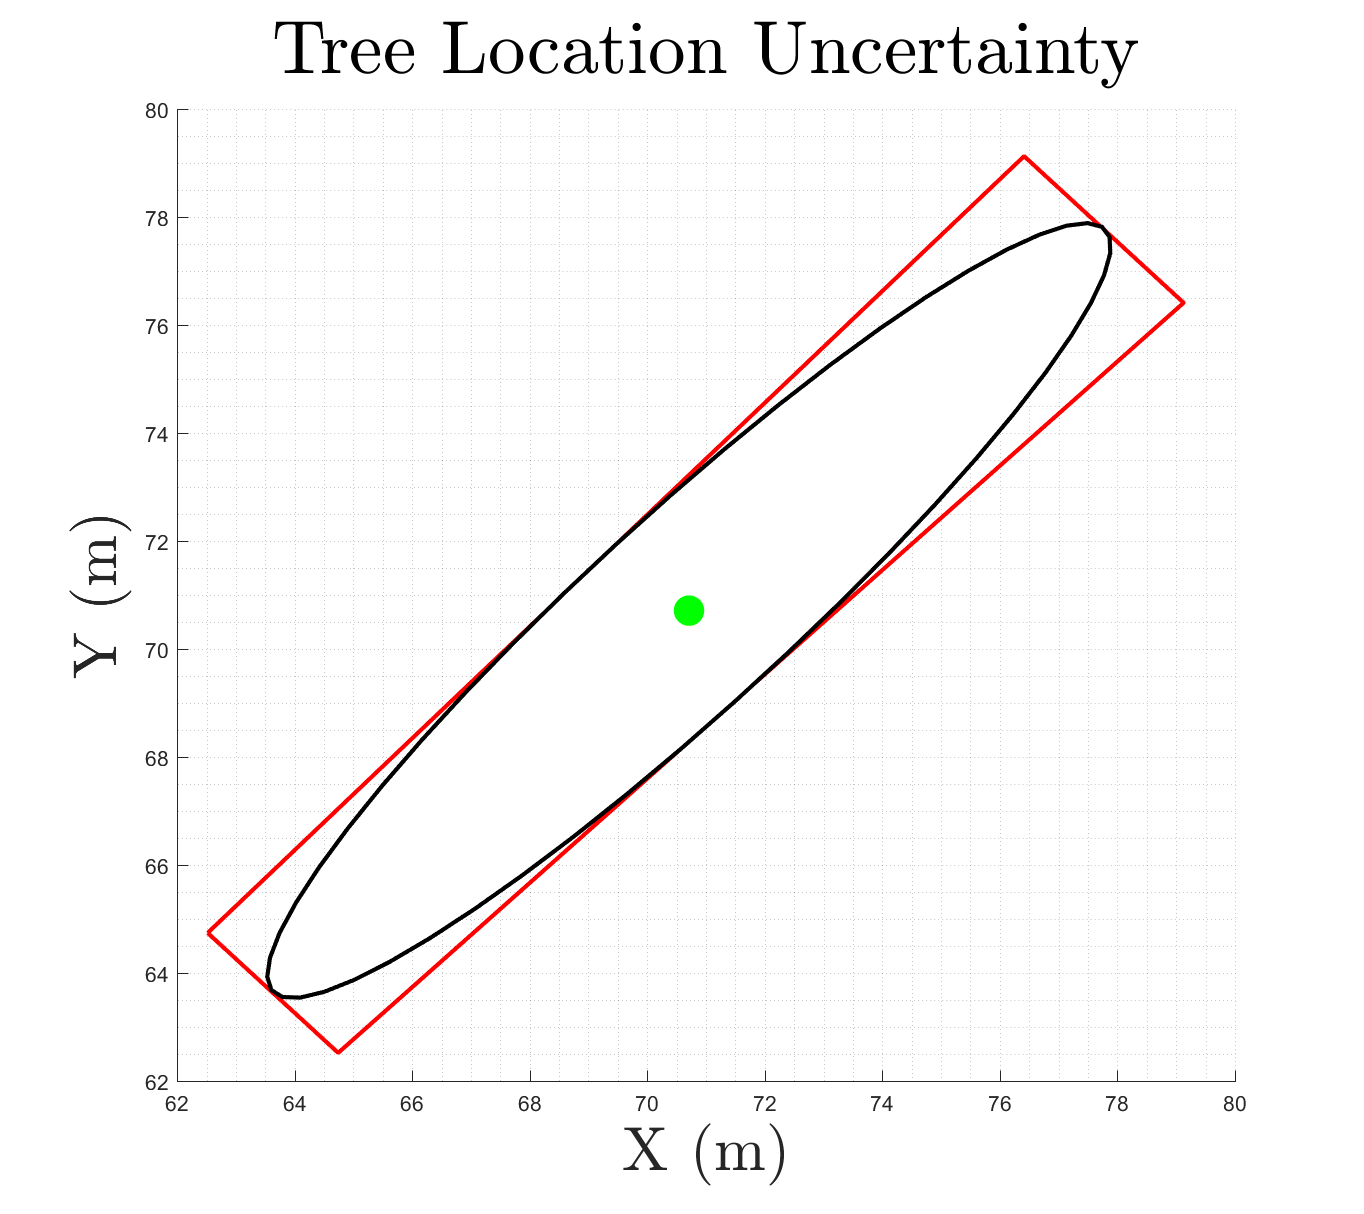
\includegraphics[height = 3in]{treefigconfidence.png}
\end{figure}

If you were to simply represent the x and y coordinate from this solution using the variance of each component, your uncertainty region would look like a rectangle.  But, this would be discarding relevant information from how the coordinate was computed.

Notice that the shape of the most probably region for the tree is an ellipse.  As the x estimate is too high, so is the y estimate.  As the x estimate is too low, so is the y estimate.  The error between the two uncertainties are correlated.  This information is what is encompassed in the covariance matrix, where the diagonal elements are the variances of each variable, and the off diagonal elements are the "covariances", which represent the correlation between the errors.  In the tree example, the covariances would be positive, as there is a positive correlation between the x and y errors.  (As the predicted X increases, the predicted Y increases)

\[
\Sigma =
\begin{bmatrix}
\sigma_{x}^2 & \sigma_{xy} \\
\sigma_{xy} & \sigma_{y}^2 \\
\end{bmatrix}
\]

The structure of a covariance matrix in a more general example looks like this:
Given three variables ($x_1,x_2,x_3$), V represents a variance, and C represents a covariance.
\[
\Sigma = 
\begin{bmatrix}
\sigma_{x_1}^2 & \sigma_{x_1x_2} & \sigma_{x_1x_3} \\
\sigma_{x_1x_2} & \sigma_{x_2}^2 & \sigma_{x_2x_3} \\
\sigma_{x_1x_3} & \sigma_{x_2x_3} & \sigma_{x_3}^2 \\
\end{bmatrix}
=
\begin{bmatrix}
V & C & C \\
C & V & C \\
C & C & V \\
\end{bmatrix}
\]

Covariance matrices must have a specific structure.  A covariance matrix must:
\begin{itemize}
	\item Be Symmetrical
	\item Be Positive Semi-Definite (positive eigen values)
	\item Have \textbf{positive} variances on the diagonal
	\item Contain Real numbers (no imaginary)
\end{itemize}